% 建议使用 XeLaTeX 或 LuaLaTeX 编译(中文与公式支持更佳)
\documentclass[UTF8,zihao=-4]{ctexart}

\usepackage[a4paper,margin=2.5cm]{geometry}
\usepackage{amsmath, amssymb, amsthm}
\usepackage{bm}
\usepackage{hyperref}
\usepackage{graphicx}
\usepackage{caption}
\usepackage{listings}
\usepackage{xcolor}
\usepackage{float}
\usepackage{placeins}
\graphicspath{{figures/}}

\lstdefinestyle{code}{
  basicstyle=\ttfamily\small,
  numbers=left,
  numberstyle=\tiny,
  numbersep=8pt,
  keywordstyle=\color{blue},
  commentstyle=\color{teal!70!black},
  stringstyle=\color{orange!70!black},
  showstringspaces=false,
  breaklines=true,
  frame=single,
  framerule=0.3pt,
  rulecolor=\color{black!15}
}
\lstset{style=code}

\title{高斯混合模型:原理、公式、应用与实战}
\author{}
\date{\today}

\begin{document}
\maketitle

\section{引言}
高斯混合模型(Gaussian Mixture Model, GMM)将数据描述为多个高斯分布的加权和,每个成分拥有独立的均值、协方差与混合系数,可解释为潜在簇。相比 K-means,GMM 能够拟合椭圆簇与重叠分布,并提供概率意义上的软分配与密度估计。

\section{原理与公式}
\subsection{混合密度函数}
对 \(\mathbf{x} \in \mathbb{R}^d\),GMM 的概率密度为
\begin{equation}
p(\mathbf{x}\,|\,\Theta) = \sum_{k=1}^K \pi_k \mathcal{N}(\mathbf{x} \,|\, \bm{\mu}_k, \mathbf{\Sigma}_k),
\end{equation}
其中 \(\Theta = \{\pi_k, \bm{\mu}_k, \mathbf{\Sigma}_k\}_{k=1}^K\),混合系数满足 \(\sum_k \pi_k = 1\)、\(\pi_k \ge 0\)。

\subsection{期望最大化算法}
常用的极大似然估计通过 EM 算法实现:
\begin{enumerate}
  \item \textbf{E 步}:利用贝叶斯公式计算责任度 \(\gamma_{ik} = p(z_i = k \,|\, \mathbf{x}_i, \Theta^{(t)})\)。
  \item \textbf{M 步}:基于责任度更新参数:
  \begin{align}
  \pi_k^{(t+1)} &= \frac{1}{n} \sum_{i=1}^n \gamma_{ik},\\
  \bm{\mu}_k^{(t+1)} &= \frac{\sum_{i=1}^n \gamma_{ik} \mathbf{x}_i}{\sum_{i=1}^n \gamma_{ik}},\\
  \mathbf{\Sigma}_k^{(t+1)} &= \frac{\sum_{i=1}^n \gamma_{ik} (\mathbf{x}_i - \bm{\mu}_k^{(t+1)})(\mathbf{x}_i - \bm{\mu}_k^{(t+1)})^\top}{\sum_{i=1}^n \gamma_{ik}}.
  \end{align}
  \item 重复迭代直至对数似然收敛。
\end{enumerate}

\subsection{模型选择}
可通过贝叶斯信息准则(BIC)或赤池信息准则(AIC)在选择成分数 \(K\) 与协方差结构(full、tied、diag、spherical)时进行复杂度惩罚。责任度提供软分配,可设阈值用于异常检测。

\section{应用与技巧}
\begin{itemize}
  \item \textbf{密度估计}:在语音、金融或传感器序列中刻画多峰分布。
  \item \textbf{软聚类}:责任度反映不确定性与重叠簇,适用于客户分群或主题识别。
  \item \textbf{异常检测}:在混合模型下似然较低的样本可视为异常事件。
  \item \textbf{实用建议}:特征需缩放,初始化可结合 K-means 与多次随机重启,监控协方差条件数,并通过正则(如加入 \(10^{-6}\)I)避免奇异矩阵。
\end{itemize}

\section{Python 实战}
脚本 \texttt{gen\_clustering\_gmm\_figures.py} 在合成数据上拟合 GMM,绘制密度等高线,并比较不同成分数的 BIC。
\begin{lstlisting}[language=Python,caption={脚本 gen_clustering_gmm_figures.py 片段}]
from sklearn.mixture import GaussianMixture

model = GaussianMixture(n_components=3, covariance_type="full",
                        init_params="kmeans", random_state=42)
model.fit(points)
responsibilities = model.predict_proba(points)

bic_scores = []
for k in range(1, 7):
    gm = GaussianMixture(n_components=k, covariance_type="full",
                         init_params="kmeans", random_state=42)
    gm.fit(points)
    bic_scores.append(gm.bic(points))
\end{lstlisting}

\section{实验结果}
\begin{figure}[H]
  \centering
  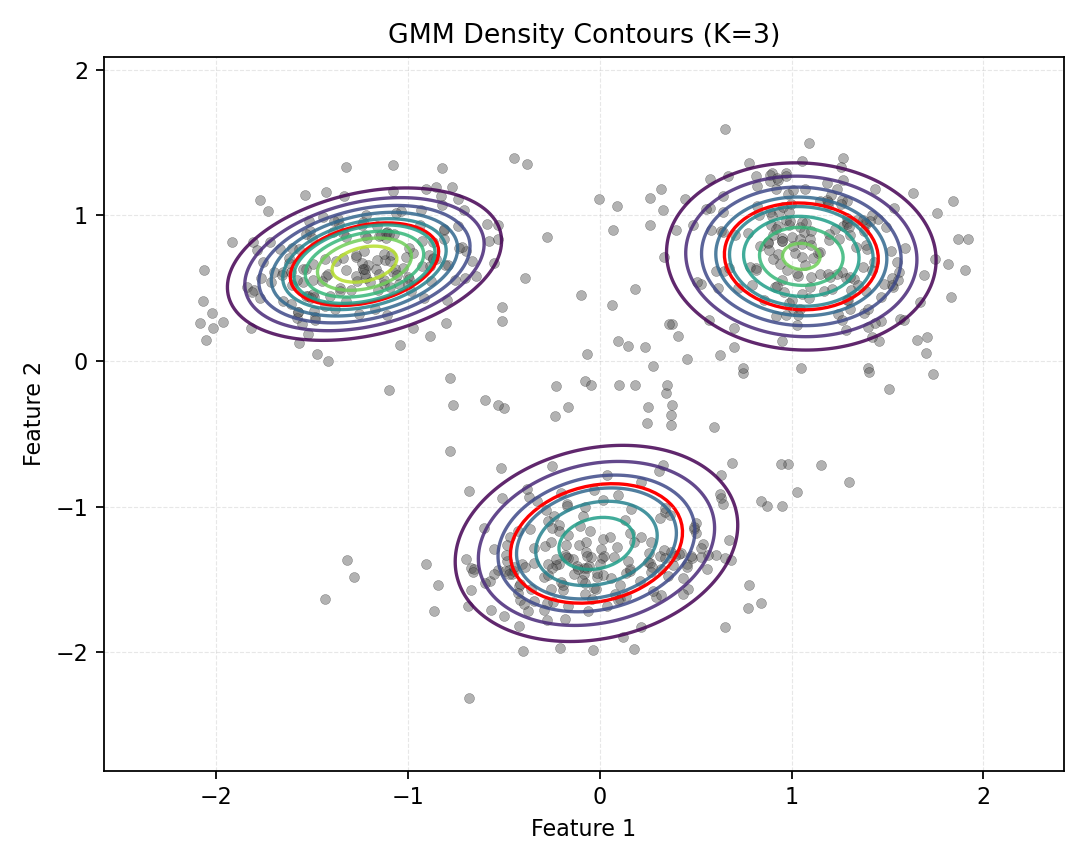
\includegraphics[width=0.82\linewidth]{gmm_density_contours.png}
  \caption{三成分 GMM 在合成数据上的密度等高线}
  \label{fig:gmm_density_contours_cn}
\end{figure}

\begin{figure}[H]
  \centering
  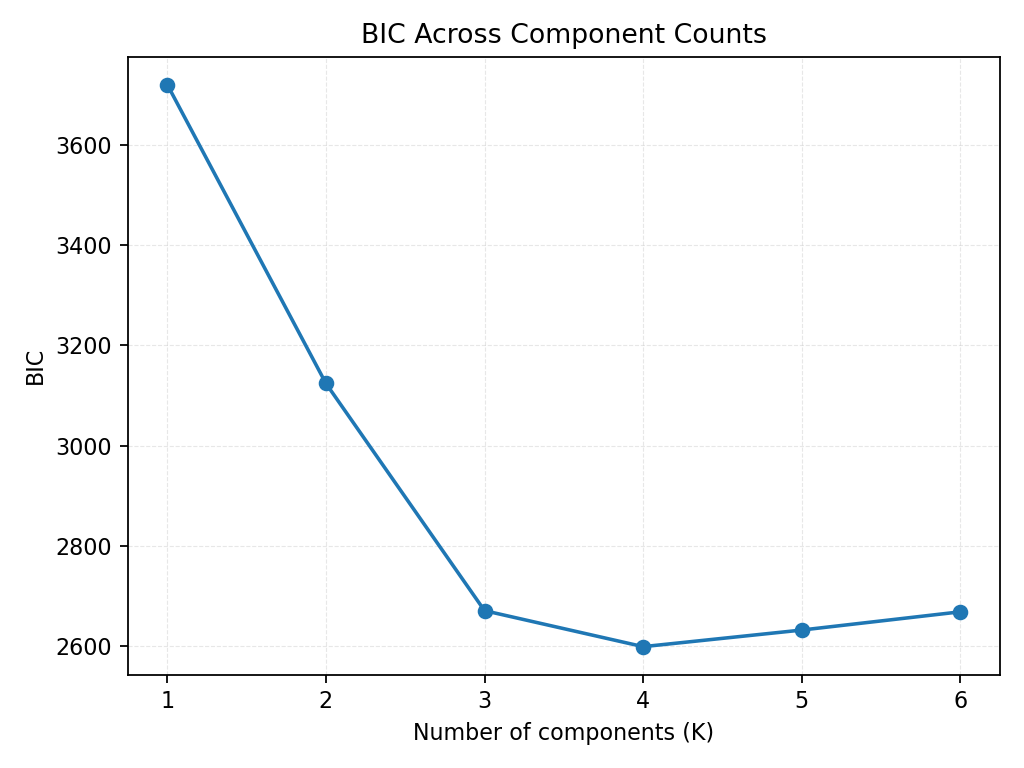
\includegraphics[width=0.8\linewidth]{gmm_bic_curve.png}
  \caption{不同成分数下的 BIC 曲线}
  \label{fig:gmm_bic_curve_cn}
\end{figure}

\FloatBarrier
\section{总结}
高斯混合模型通过刻画协方差结构与概率分配拓展了 K-means。EM 算法在责任度与参数更新之间迭代直至收敛;借助 BIC 等指标可评估成分数并识别奇异解。示例展示了密度可视化与模型选择如何互补,指导实际应用。

\end{document}
